\begin{lovkapittel}{Generelt arbeidsreglement for ansatte}


    \begin{lovparagraf}{Gyldighet og omfang}
        Arbeidsreglementet er vedtatt av Finansstyret ved Studentersamfundet i Trondhjem og gjelder alle arbeidstakere i et
        fast forpliktende arbeidsforhold ved Studentersamfundet i Trondheim.
        Reglene i reglementet gjelder ikke når de strider mot lov, tariffavtale eller andre bestemmelser som er bindende for
        Studentersamfundet.
    \end{lovparagraf}

    \begin{lovparagraf}{Ansettelser}
        Alle arbeidstakere blir ansatt av daglig leder. Når arbeidstakeren tiltrer skal denne forelegges arbeidsavtale som både
        arbeidsgiver og arbeidstaker skriver under på.

        Daglig leder blir tilsatt av Finansstyret.
    \end{lovparagraf}

    \begin{lovparagraf}{Legeattest}
        For stillinger hvor det stilles spesielle krav til helse, skal det før ansettelser framlegges tilfredsstillende legeattest.
    \end{lovparagraf}

    \begin{lovparagraf}{Ferie}
        Ferien ordnes i samsvar med reglene i gjeldende ferielov og tariffavtale.

        Arbeidsgiver fastsetter ferietid etter konferanse med arbeidstakeren eller vedkommendes tillitsvalgte. Ferielisten skal
        som hovedregel gjøres kjent tidligst mulig og senest 2 måneder før ferien tar til.
    \end{lovparagraf}

    \begin{lovparagraf}{Utbetaling av lønn}
        Måneds- og årslønte utbetales lønn etterskuddsvis den 15. i måneden eller nærmeste foregående virkedag.

        Når særlig grunn foreligger, kan det utbetales forskudd med inntil halvparten av ordinær netto månedslønn. Eventuelt
        forskudd utbetales kun en gang pr. mnd.- den 30.

        Time-, dag- og ukelønte utbetales lønn etterskuddsvis den 15. i påfølgende måned. Den enkelte arbeidstaker skal kontrollere at det er utbetalt riktig beløp. Eventuell feil må meldes snarest mulig.

        Fradrag i lønningene kan ikke gjøres unntatt i følgende tilfeller:

        \begin{enumerate}
            \item Lovbestemte trekk.
            \item Pensjonsinnskudd. Pensjonsinnskudd trekkes fra tiltredelsesdato.
            \item Beløp som på forhånd er skriftlig avtalt mellom Studentersamfundet og arbeidstakeren.
            \item Erstatning for skade eller tap arbeidstakeren forsettlig eller grovt uaktsom har påført 
                Studentersamfundet. Betingelsen for slikt trekk er at arbeidstakeren skriftlig erkjenner 
                erstatningsansvar, eller det er fastslått ved dom, eller arbeidstakeren rettsstridig fratrer 
                sin stilling. Lønnstrekk skal begrenses til den del av lønnen som overstiger det arbeidstakeren 
                med rimelighet trenger til underhold for seg og sin husstand. Før trekk etter pkt. d, 
                gjennomføres, skal det konfereres med arbeidstakerens tillitsvalgte.  
        \end{enumerate} 
    \end{lovparagraf}

    \begin{lovparagraf}{Fravær fra arbeidet}
        Fravær på grunn av sykdom, ulykke eller andre årsaker skal så snart som mulig meddeles nærmeste overordnede.

        For sykefravær til og med 8 etterfølgende arbeidsdager skal det leveres egenmelding. Arbeidstakeren plikter ikke å gi
        opplysning om sykdommens art.

        Arbeidsgiver kan kreve legeattest fra første dag dersom arbeidstakeren i de siste 12 måneder har hatt flere enn 4
        kortvarige fravær. Det samme gjelder ved gjentatte sykefravær færre enn 4 ganger dersom arbeidsgiver har rimelig
        grunn til å anta at fraværet ikke skyldes sykdom.

        Før arbeidstakeren mister retten til å nytte egenmelding, skal vedkommende gis anledning til å redegjøre for årsaken
        til at det har vært så mange fravær.

        Ved lengre fravær enn 8 etterfølgende arbeidsdager skal det leveres legeattest. 
    \end{lovparagraf}

    \begin{lovparagraf}{Alminnelig orden}
        Arbeidstakeren må være på arbeidsstedet/mønstringsstedet ved arbeidstidens begynnelse.
        Ingen må forlate arbeidsstedet i arbeidstiden uten tillatelse.

        Arbeidstakeren må ikke være påvirket av alkohol eller annet berusende eller bedøvende middel i arbeidstiden.
    \end{lovparagraf}

    \begin{lovparagraf}{Behandling av utstyr}
        Alt inventar, maskiner, verktøy, materialer m.v. må behandles med omhu. Det må vises forsiktighet ved behandlingen
        av ild, lys og ildsfarlige saker.

        Arbeidstakeren må behandle Studentersamfundets utstyr m.v. med størst mulig varsomhet, slik at ødeleggelse og
        unødvendig slitasje ikke oppstår.

        Ved uforsiktig omgang med materiell kan arbeidstakeren pålegges erstatningsansvar.

        Studentersamfundet plikter etter lov og forskrifter å stille til rådighet verneutstyr der dette er påkrevd. Arbeidstakeren
        plikter på samme måte, for å trygge liv, helse og eiendom å bruke det verneutstyr som er stilt til disposisjon, jfr.
        Arbeidsmiljøloven § 16.

        Likeledes plikter arbeidstakeren å ta vare på utlevert verneutstyr og rapportere til overordnet når det måtte oppstå
        eventuelle feil eller mangler ved utstyret.
    \end{lovparagraf}

    \begin{lovparagraf}{Permisjon}
        For permisjon gjelder Arbeidsmiljølovens bestemmelser.
    \end{lovparagraf}

    \begin{lovparagraf}{Oppsigelse}
        Oppsigelsen skal være skriftlig fra begge parter. Blir arbeidstakeren oppsagt, kan hun/han kreve skriftlig begrunnelse
        for oppsigelsen.

        Ved oppsigelse fra Studentersamfundet skal denne inneholde opplysninger om arbeidstakerens rett til å kreve
        forhandlinger, reise søksmål, og hvilke frister som gjelder. Før slik oppsigelse finner sted, skal det konfereres med
        arbeidstakerens tillitsvalgte.

        Oppsigelsesfristene skal være i samsvar med gjeldende bestemmelser i lov og tariffavtale.

        Om arbeidstakernes rettigheter ved oppsigelse, vises forøvrig til Arbeidsmiljølovens kapittel XII og
        Forvaltningslovens bestemmelser.

        Ved fratredelse har arbeidstakeren krav på sluttattest.
    \end{lovparagraf}

    \begin{lovparagraf}{Avskjed}
        Arbeidsgiver kan avskjedige en arbeidstaker med påbud om øyeblikkelig fratreden dersom denne har gjort seg skyldig
        i grovt pliktbrudd eller annet vesentlig mislighold av arbeidsavtalen.

        Avskjeden skal meddeles skriftlig og inneholde opplysninger om rett til å kreve forhandling, reise søksmål og hvilke
        frister som gjelder.

        (Mens spørsmål om avskjed behandles, kan arbeidstakeren i helt spesielle tilfeller suspenderes fra sin stilling.
        Betingelsen for å kunne foreta suspensjon er at det er nødvendig av hensyn til tjenestens art at arbeidstakeren straks
        blir fjernet fra sin nåværende stilling, og at det må være grunn til å anta at vilkårene for avskjed etter
        Arbeidsmiljølovens § 66 nr.1 er til stede.)

        Arbeidstakeren har krav på å få beholde sin lønn inntil vedtak om avskjed er truffet.
        Før vedtak om avskjed eller suspensjon treffes, skal det konfereres med arbeidstakerens tillitsvalgte med mindre
        arbeidstakeren selv ikke ønsker dette. Ved suspensjon har arbeidstakeren krav på at denne blir begrunnet.

        Om arbeidstakerens rettigheter forøvrig vises til Forvaltningsloven, i spørsmål om avskjed vises også til
        Arbeidsmiljølovens § 57 (oppsigelse), jfr. § 66.
    \end{lovparagraf}

    \begin{lovparagraf}{Informasjon til media}
        Studentersamfundets ansatte må innhente fullmakt hos daglig leder for å gi opplysninger til media.

    \end{lovparagraf}

    \begin{lovparagraf}{Taushetsplikt}
        Når en sak er undergitt taushetsplikt i henhold til lov, andre bestemmelse, eller når det følger av sakens art, må ingen
        arbeidstaker omtale saken overfor noen utenforstående.
    \end{lovparagraf}

    \begin{lovparagraf}{Fortolkning/tvist}
        Tvist om fortolking av dette reglement behandles av daglig leder og ansattes tillitsvalgte. Endringer i reglementet kan
        foretas i Finansstyret etter forslag fra daglig leder eller ansattes tillitsvalgte.
    \end{lovparagraf}
\end{lovkapittel}


\begin{instruks}{Stillingsinstruks for Daglig Leder}{9. april 2002}{9. april 2002}
    \begin{instruksledd}{Beskrivelse}
        \begin{enumerate}
            \item Stillingen er underlagt Finansstyret. Til daglig er Finansstyrets leder kontaktperson for daglig leder.
            \item Daglig leder leder Studentersamfundets forretningsmessige virksomhet og har ansvar for menneskelige og materielle
                ressurser. Daglig leder skal virke innen rammene gitt av Studentersamfundets lover og retningslinjer vedtatt av FS.
            \item Daglig leder kan avgjøre alle saker og forplikte Studentersamfundet innenfor de fullmakter som FS til enhver tid har
                fastsatt gjennom sine vedtak. I saker som er av en slik karakter eller størrelse at de går ut over daglig leders
                fullmakter skal saken forelegges FS for beslutning. Avtaler o.a. som følger av foregående ledd skal signeres
                av både leder av FS og daglig leder.
            \item Daglig leder har anvisningsmyndighet for Studentersamfundet og arbeidsgiveransvar for Studentersamfundets ansatte.
        \end{enumerate}
    \end{instruksledd}

    \begin{instruksledd}{Hovedoppgaver}
        \begin{enumerate}
            \item Daglig leder skal:
                \begin{itemize}
                    \item sørge for at Studentersamfundet har en administrativ organisasjon med den kompetanse som til
                        enhver tid kreves for at Studentersamfundet skal nå sine mål.
                    \item sørge for tilfredsstillende forvaltning, drift og vedlikehold av Studentersamfundets eiendommer.
                    \item ivareta og utvikle utleievirksomheten.
                    \item utarbeide budsjetter og regnskap etter gjeldende lover og forskrifter
                    \item støtte foreninger og gjenger i gjennomføringen av administrative oppgaver, hovedsakelig innen
                        regnskap, forvaltning av likvider og varelager.
                    \item ivareta kontakt med offentlige myndigheter.
                \end{itemize}
            \item Daglig leder er skjenkebestyrer for Studentersamfundets skjenkebevilgning.
        \end{enumerate}
    \end{instruksledd}

    \begin{instruksledd}{Ansatte}
        \begin{enumerate}
            \item Alle ansatte ved Studentersamfundet er underlagt daglig leder med mindre annet er vedtatt 
                i FS. Daglig leder er ansvarlig for
                ansettelser og de ansattes arbeidsforhold. Daglig leder fastlegger de ansattes arbeids- og ansvarsområde. Vesentlige
                organisasjonsendringer fremmes for FS.
        \end{enumerate}
    \end{instruksledd}
\pagebreak
    \begin{instruksledd}{Foreningsdrift og Gjenger}
        \begin{enumerate}
            \item Studentersamfundet drives i hovedsak av frivillige. Daglig leder skal sørge for at den administrative organisasjonen
                støtter opp om foreningsdriften og gjengenes virksomhet.
        \end{enumerate}
    \end{instruksledd}

    \begin{instruksledd}{Finansstyret}
        \begin{enumerate}
            \item Daglig leder har møte- og talerett i FS. Daglig leder kaller inn til FS møter. Daglig leder 
                forbereder og framlegger saker vedrørende
                forretningsdriften og områder som berøres av denne instruksen. Daglig leder rapporterer regelmessig nøkkeltall og
                økonomiske resultater til FS. Daglig leder gjennomfører vedtak fattet i FS.
            \item Daglig leder holder arkiv over korrespondanse i samband med forretningsdriften. Videre holdes arkiv for FS og Rådet
                i samarbeid med Studentersamfundets arkivarer.
        \end{enumerate}
    \end{instruksledd}

    \begin{center}
    	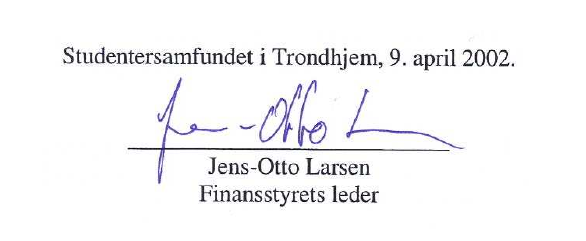
\includegraphics[width=0.5\textwidth]{DagligLeder-sign}
    \end{center}

\end{instruks}


\begin{instruks*}{Stillingsinstruks for vaktmester}
    \begin{instruksledd}{Stillingen}
        \begin{enumerate}
            \item Vaktmester er underlagt daglig leder.
        \end{enumerate}    
    \end{instruksledd}

    \begin{instruksledd}{Ansvarsområde}
        \begin{enumerate}
            \item Ansvarlig for det daglige tilsyn av Studentersamfundets bygninger.
            \item Påse at forsvarlig vedlikehold blir utført
            \item Vaktmester er avdelingsleder for vakter/garderobepersonale. For å administrere dette avsettes det 2 dager pr.
                måned.
            \item Vaktmester innstiller personer til vakter/garderobepersonale, overfor daglig leder.
            \item Vaktmester står ansvarlig for vekselkasse i garderoben
            \item Vaktmester har oppfølgingsansvar for nødvendig vedlikehold for daglig drift
            \item Vaktmester er Brannvernansvarlig ved Studentersamfundet i Trondhjem
        \end{enumerate}    
    \end{instruksledd}

    \begin{instruksledd}{Myndighetsområde}
        \begin{enumerate}
            \item Vaktmester disponerer vedlikeholdsmidler i henhold til budsjett, og etter avtale med daglig leder
            \item Vaktmester har innstillingsrett i vedlikeholdssaker og saker vedrørende brann og el.sikkerhet overfor daglig
                leder
            \item Vaktmester har myndighet til å delegere nødvendige vedlikeholdsoppgaver til Diversegjengen
        \end{enumerate}
    \end{instruksledd}

    \begin{instruksledd}{Arbeidsoppgaver}
        \begin{enumerate}
            \item Tilsyn med fyring og ventilasjonsanlegg
            \item Tilsyn med det elektriske anlegget
            \item Vedlikehold av dører og vinduer
            \item Tilsyn med Studentersamfundets heiseanlegg
            \item Tilsyn med brannvernrutiner ved Studentersamfundet i Trondhjem i samråd med daglig leder og Sikringssjef
            \item Ansvarlig for forefallende reparasjonsarbeid
            \item Vedlikehold/reparasjon av inventar
            \item Flagging på offentlige høytidsdager, Studentersamfundets festdager og ellers når Styret eller daglig leder gir
                beskjed   
        \end{enumerate}
    \end{instruksledd}

    \begin{instruksledd}{Arbeidstid}
        \begin{enumerate}
            \item 37,5 timers arbeidsuke. Kjernetid mellom klokken 09.00 og 15.00. Øvrig arbeidstid fordeles av vaktmester
                etter behov. 
        \end{enumerate}
    \end{instruksledd}

\end{instruks*}



\begin{instruks*}{Instruks for dørvakter}
    \begin{instruksledd}{Stillingen}
        \begin{enumerate}
            \item Stillingen er underlagt daglig leder som er ansvarlig for Studentersamfundets forretningsmessige virksomhet.
            \item Vakter ansettes av daglig leder etter anbefaling fra vaktmester. Vaktmester er dørvaktenes 
                overordnede og de er direkte underlagt vaktmester.
        \end{enumerate}    
    \end{instruksledd}

    \begin{instruksledd}{Ansvarsområde}
        \begin{enumerate}
            \item Lønn og eventuelle andre godtgjørelser fastsettes av Finansstyret.
            \item Arbeidet er sesongbetont og følger semestrene ved NTNU.
            \item Vakter og vaktleder vil bli innkalt etter behov.
            \item Arbeidstiden for faste arrangement, er for tiden innenfor disse tidsrammene:
                \begin{itemize}
                    \item Klubbaften 20.30--04.00
                    \item Lørdagsmøte 18.00--04.00
                \end{itemize}
            \item Pause er inkludert i arbeidstiden.
            \item Andre arrangementer vil variere i varighet.
            \item For hvert arrangement skal det være en vaktleder. Denne utnevnes av vaktmester.
            \item Vaktmester er kontaktperson for dørvakter.
            \item Vaktleder er dørvaktenes nærmeste overordnede og han/hun er den personen som har et overordnet ansvar i
                forhold til de ansatte under arrangementet. Vaktleder rapporterer til vaktmester.
            \item Vakter stiller i arbeidsantrekk stilt til rådighet av Studentersamfundet i Trondhjem.
        \end{enumerate}    
    \end{instruksledd}

    \begin{instruksledd}{Hovedoppgaver}
        \begin{enumerate}
            \item Vakter skal opptre korrekt og være serviceinnstilt overfor Studentersamfundets gjester.
            \item Vakter skal opprettholde ro og orden ved Studentersamfundets arrangementer.
            \item Vakter skal kontrollere medlemskort, inngangsbilletter og alderslegitimasjon.
            \item Vakter skal kontrollere at bestemmelsene i skjenkeloven overholdes.
            \item Vakter plikter å gjøre seg kjent med branninstruks, brannsentral, Sprinkleranlegg, Studentersamfundets
                organisasjonsstruktur, deler av det tekniske anlegget og lokalisering av hovedvannkran.
            \item Vakter skal bistå arrangør ved ulike problemer som måtte oppstå.
            \item Vakter skal om mulig bistå Serveringsgjengen ved tekniske problemer.
            \item Vakter skal bistå garderoben ved stor pågang.
            \item Under selve arrangementet bør vakta så langt det er mulig være arrangør behjelpelig med å rydde, etterfylle
                papir på toalettene osv.
            \item Det bør alltid stå minst to vakter i døra, med unntak av når vakta er tilkalt på nødvendig oppdrag.
            \item Vakter skal kunne grunnleggende førstehjelp. Førstehjelputstyr skal være tilgjengelig.
            \item Vaktleder skal sørge for veksel til garderoben, og kontrollere oppgjøret ved arrangementets slutt. 
            \item Vaktleder har myndighet til å anmelde personer til politiet, når vaktleder mener dette er nødvendig.
        \end{enumerate}
    \end{instruksledd}

    \begin{instruksledd}{Foreningsdrift og gjenger}
        \begin{enumerate}
            \item Vakter og vaktleder skal samarbeide med arrangerende gjeng (KLST/LK/KU ev. andre arrangører). De skal
                også gjøre seg kjent med arrangørinstruksen for arrangementet. Dette for å kunne yte god service til
                Studentersamfundets gjester.
            \item Vakter har ikke adgang til å slippe inn personer gratis, uten å ha avklart dette med arrangerende gjeng.
            \item Vakter og vaktleder skal samarbeide med barsjefer. Ved eventuelle konflikter angående berusede personer
                osv. skal dette avgjøres av vaktleder og gjeldende barsjef.
        \end{enumerate}    
    \end{instruksledd}

    \begin{instruksledd}{Andre forhold}
        \begin{enumerate}
            \item Vakter har utenfor arbeidstid adgang til arrangementer ved Studentersamfundet i ordinær åpningstid. De
                ansatte blir da regnet som vanlige gjester på huset. Det tilligger likevel ansatte ved Studentersamfundet et
                særlig ansvar for å opptre innenfor rammene av god oppførsel.
            \item Ved arbeidets slutt har dørvakter adgang til de private områdene. Adgang til de private områdene for følger
                oppnås kun etter avtale med en av gjengene. 
        \end{enumerate}
    \end{instruksledd}
\end{instruks*}

\begin{instruks*}{Instruks for garderobevakter}
    
    \begin{instruksledd}{Stillingen}
        \begin{enumerate}
            \item Stillingen er underlagt daglig leder som er ansvarlig for Studentersamfundets forretningsmessige virksomhet.
                Garderobevakter ansettes av daglig leder etter anbefaling fra vaktmester. Vaktmester er garderobevaktenes nærmeste
                overordnede og de er direkte underlagt vaktmester.
        \end{enumerate}    
    \end{instruksledd}

    \begin{instruksledd}{Lønns- og arbeidsvilkår}
        \begin{enumerate}
            \item Lønn og eventuelle andre godtgjørelser følger Norsk Arbeidsmannsforbunds tariffer.
            \item Arbeidet er sesongbetont og følger semestrene ved NTNU.
            \item Garderobevakter vil bli innkalt etter behov.
            \item Arbeidstiden for faste arrangement, er for tiden innenfor disse tidsrammene:
                \begin{itemize}
                    \item Klubbaften 20.30--04.00
                    \item Lørdagsmøte 18.00--04.00
                \end{itemize}
            \item Pause er inkludert i arbeidstiden.
            \item Andre arrangementer vil variere i varighet.
            \item Garderobepersonalet stiller i arbeidsantrekk stilt til rådighet av Studentersamfundet i Trondhjem.
        \end{enumerate}    
    \end{instruksledd}

    \begin{instruksledd}{Hovedoppgaver}
        \begin{enumerate}
            \item Garderoben er et av Studentersamfundets servicetilbud, og er en del av vår fasade 
                utad mot publikum. Det er derfor garderobe personalets viktigste oppgave å være serviceinnstilt og 
                imøtekommende overfor gjestene.
            \item Personalet er i arbeidstiden ansvarlig for innhengt tøy.
            \item Gjenglemt tøy samles og henges i garderoben ved arrangementets slutt.
            \item Garderobevakter er ansvarlig for at riktig garderobeoppgjør blir levert vaktleder.
        \end{enumerate}
    \end{instruksledd}

    \begin{instruksledd}{Foreningsdrift og gjenger}
        \begin{enumerate}
            \item Garderobevakter skal samarbeide med arrangerende gjeng (KLST/LK evt. andre arrangører). De skal også gjøre seg
                kjent med arrangørinstruksen for arrangementet. Dette for å kunne yte god service til Studentersamfundets gjester.
        \end{enumerate}
    \end{instruksledd}

    \begin{instruksledd}{Andre forhold}
        \begin{enumerate}
            \item Garderobevakter har utenfor arbeidstid adgang til arrangementer ved Studentersamfundet i ordinær åpningstid. De
                ansatte blir da regnet som vanlige gjester på huset. Det tilligger allikevel ansatte ved Studentersamfundet et særlig
                ansvar for å opptre innenfor rammene av god oppførsel.
            \item Ved arbeidets slutt har garderobevakter ikke adgang til de private områdene Adgang til de private områdene oppnås
                kun etter invitasjon fra en av gjengene. Invitasjonen og adgangen til de private områdene skal også klareres med
                Husmann i hvert enkelt tilfelle.
        \end{enumerate}
    \end{instruksledd}

\end{instruks*}

